\documentclass[a4paper]{article}

\usepackage[margin=1in]{geometry}  % redefine document margins
\usepackage[authoryear]{natbib}    % use author-year reference type
\usepackage{float}                 % improves the interface for defining floating objects
\usepackage{caption}               % customise the captions in figures and tables
\usepackage{subcaption}            % similar to caption but for subfigures
\usepackage{graphicx}              % add optional arguments to \includegraphics
\usepackage{multirow}              % provide multirow table capability
\usepackage{hyperref}              % cross-referencing support
\usepackage{booktabs}              % publication quality tables
\usepackage{siunitx}               % provide std uncertainty next to means
\usepackage{tabularx}              % allows text wrapping in table cells

% configurations necessary for table2
\sisetup{table-align-uncertainty,separate-uncertainty}
\newcolumntype{Y}{S[detect-weight,mode=text]}
\renewrobustcmd{\bfseries}{\fontseries{b}\selectfont}

% make caption font size smaller
\captionsetup[figure]{font=small,labelfont=small}


\title{MapIntel: Enhancing Competitive Intelligence Acquisition Through Embeddings and Visual Analytics}
\author{David Silva, Fernando Bação}
\date{}

\begin{document}
\maketitle

\begin{abstract}
	Competitive Intelligence allows an organization to keep up with market trends and foresee business opportunities. This practice is mainly performed by analysts scanning for any piece of valuable information in a myriad of dispersed and unstructured sources. Here we present MapIntel, a system for acquiring intelligence from vast collections of text data by representing each document as a multidimensional vector that captures its own semantics. The system is designed to handle complex Natural Language queries and visual exploration of the corpus, potentially aiding overburdened analysts in finding meaningful insights to help decision-making. The system \emph{searching} module uses a retriever and re-ranker engine that first finds the closest neighbors to the query embedding and then sifts the results through a cross-encoder model that identifies the most relevant documents. The \emph{browsing} or visualization module also leverages the embeddings by projecting them onto two dimensions while preserving the multidimensional landscape, resulting in a map where semantically related documents form topical clusters which we capture using topic modeling. This map aims at promoting a fast overview of the corpus while allowing a more detailed exploration and interactive information encountering process. We evaluate the system and its components on the 20 newsgroups dataset, using the semantic document labels provided, and demonstrate the superiority of Transformer-based components. Finally, we present a prototype of the system in Python and show how some of its features can be used to acquire intelligence from a news article corpus we collected during a period of 8 months.
\end{abstract}

\section{Introduction}
% Introducing the topic: Opening with a strong opening hook
Competitive Intelligence (CI) is the process and forward-looking practices used in producing knowledge about the competitive environment to improve organizational performance \citep{madureira2021}. According to \citet{brod1999}, "Companies with competitive intelligence programs have better knowledge of their markets, better cross-functional relationships between their business units and a greater ability to develop proactive competitive strategies." CI has a fundamental role in helping businesses remain competitive, influencing a wide range of decision-making areas, and leading to substantial improvements such as the increase of revenue, new products or services, cost savings, time savings, profit increases, and achievement of financial goals \citep{calof2017}.

% Making the case and defining the goal of the paper
Competitive Intelligence analysts are responsible for developing the CI task through a combination of gathering data, processing it, and communicating information. The digitalization of the market and the growth of the data economy have pushed the business environment to an online realm where every action and event is public and thus potentially relevant for decision-making. This shift has produced a large volume of data about products, customers, competitors, and any aspect of the business environment that can be used to foresee opportunities and risks. Given the vastness and diversity of this data, it has become necessary to design tools that can aid analysts in the CI gathering and analysis process. Therefore, the goal is to enhance the analyst's task by providing a means to explore, organize and visualize the environmental data present in the array of existing sources.

Traditionally, the most important sources of CI have been news providers, corporate websites, and trade publications, respectively \citep{marin2004}. With the advent of the internet, new sources, such as social networks \citep{dey2011}, have emerged, while existing ones have become enriched and easily accessible. Despite the increased availability, CI resources are dispersed through a variety of websites and the underlying data is unstructured and noisy. These characteristics add to the difficulty of the analyst's task and exacerbate the need for tools to support it.

% Describe the background: an overview of the most relevant research that has already been conducted (what has been done and what are the limitations that we intend to explore)
Various studies have attempted to create systems for exploring and gathering intelligence from extensive collections of textual data \citep{dey2011, esteva2020, lafia2019, lafia2021a, caillou2021}. These studies have consistently applied Natural Language Processing (NLP) techniques to help users comprehend large volumes of text without requiring to sift through every document. \citet{dey2011} designed a system for CI that captures data from multiple sources, cleans it, uses NLP to identify and tag the relevant content, stores it, generates consolidated reports, and produces alerts on predefined triggers.

% Establish your research problem: clarify how your own research fits in and what problem it addresses
Although the previously mentioned systems have been used for dealing with large amounts of text successfully, insufficient attention has been paid to the exploratory and serendipitous aspects of the analyst's task. Accordingly, we propose an information environment that supports analysts in having stimulating and productive information encounters. Thus, contrarily to previous systems, we center ours around Information Encountering which is defined by \citet{erdelez2020} to encompass "finding interesting, useful or potentially useful information when looking for some other information, not looking for any information in particular, or not looking for information at all." This is achieved by incorporating two types of information acquisition tasks: \emph{searching}, consisting of an information retrieval module that allows \emph{ad hoc} queries on the entire document collection, giving the user the ability to seek information actively, and \emph{browsing}, consisting of a visualization module that equips the user with tools to actively or passively acquire information through the visual exploration of the document corpus (and its thematic cohorts) in a two-dimensional map.

% Talk about the recent advent of the transformers as a justification for this system and as a distinguishing factor
With the recent emergence of the Transformer architecture \citep{vaswani2017}, significant improvements were made in several NLP subdomains, having reached state-of-the-art results in a wide range of tasks \citep{vaswani2017}. This new architecture is based solely on the attention mechanism, providing parallelization capabilities and thus avoiding the sequential nature of existing Recurrence models \citep{hochreiter1997, cho2014}. The attention mechanism allows incorporating information from the input sequence words into the one it is currently being processed, thus providing "context" to the word from the rest of the sequence. Language models like Bidirectional Encoder Representations from Transformers (BERT) \citep{devlin2019} leverage this architecture, making up a large part of the modern NLP landscape by providing a powerful off-the-shelf way to create state-of-the-art models for a wide range of tasks. The Transformer flexibility, allied to its reduced training times and improved ability to learn long-range relationships between terms in a sequence, make it one of the pillars of modern NLP research, and we intend to apply this architecture in our work.

% Specify your objective(s): what you intend to find out or express in your paper
This paper explores Transformer-based models for representing documents as semantic vectors. These vectorial representations are commonly denominated as embeddings, and we intend to use them in a CI system as a mechanism for extracting information from environmental data. Furthermore, the system facilitates Information Encountering by incorporating \emph{searching} and \emph{browsing} mechanisms that leverage the document embeddings. We have named the proposed system MapIntel which derives from (Competitive) Intelligence Map.

\section{Related Work}
% Introduction: The introduction should clearly establish the focus and purpose of the literature review.
The process of extracting business-related information for anticipating risks and opportunities is an important task for many companies, yet analysts are overwhelmed with extensive amounts of unstructured data. To support CI analysts, we propose an NLP system for exploring and gathering intelligence from large collections of textual data. To situate our contribution, we review existing work on similar systems applied in CI as well as in other domains, in this section.

% Body: Summarize and synthesize, Analyze and interpret, Critically evaluate, write in well-structured paragraphs
Early work on visualizing and interpreting large collections of documents can be found in \citet{kaski1998}, where WEBSOM - a system that organizes a document collection using Self Organizing Maps (SOM) \citep{Kohonen1982}, mapping each document into the node of a two-dimensional grid that best represents it, thus providing a reliable and visual representation of the collection - is presented. An improved version of the system is given in \citet{kohonen2013}, where users can perform queries using either a set of keywords or a descriptive sentence, a zooming feature to explore specific regions of the map with finer detail is provided and, when selecting a particular node in the map, the titles of the corresponding documents are displayed. \citet{lafia2019} also used SOM together with Latent Dirichlet Allocation (LDA) \citep{blei2003} to convey the relatedness of research themes in a multidisciplinary university library. Documents are represented as random mixtures over latent topics, where each topic is characterized by a distribution over words. That said, each document is embedded in a vector space of \emph{n} dimensions, corresponding to the number of topics selected. SOM produces a landscape for exploring the topic space and provides users with an overview of the document collection and the ability to navigate, discover items of interest, change the level of detail, select individual documents and discover relationships between documents.

Arguably, the closest method to ours in terms of domain application is \citet{dey2011}. They formulated a system for acquiring competitive intelligence from different web resources, including social media, using a wide array of text mining techniques. They also showed how the system can be integrated with the business data and adopted for future decision-making. Their goal is to help the analyst in the task of reading, extracting information, and organizing the data. The system is composed of four distinct modules: \emph{content acquisition and assimilation} gather and extract relevant content from an array of sources, \emph{data pre-processing} is responsible for cleaning and extracting relevant content from different sources, \emph{content processing} identifies and tags the relevant content from the vast collection, and \emph{alerting} notifies the user on predefined triggers such as a competitor's product launch. The paper presents an approach for labeling news articles according to CI-related topics by applying LDA clustering and extracting entities and relations within each cluster, which are then used to define the respective labels. The labeling contributes to the organization of the collection and facilitates the information extraction process.

\citep{lafia2021a} proposed a method for modeling and mapping topics from bibliometric data and built a web application based on this method. The produced map allows users to read a body of research "at a distance" while providing multiple levels of detail of the documents' topics. They also incorporated a time dimension, allowing users to understand the evolution of the topics over time. They applied Non-negative Matrix Factorization \citep{lee1999} to discover the underlying topics in the data and obtain vectorial representations of the documents, and they employ t-distributed Stochastic Neighbor Embedding (t-SNE) \citep{vandermaaten2008} for visualizing the documents, resulting in a two-dimensional representation of the corpus. To allow for different detail levels, the authors produced two maps: a coarse map of 9 topics that gives a general overview of the topics within the data and a detailed map of 36 topics that captures more specific research themes. The web application consists of an interactive dashboard that allows users to explore the map of documents and easily extract information.

We based our \emph{searching} module on the Vector Space Model (VSM) \citep[p.~120-126]{schutze2008}, a common framework in Information Retrieval, consisting of representing a set of documents as vectors in a vector space while also allowing full-text queries to be represented in the same space. The model then ranks each document in decreasing order of their similarity with the query. The fundamental assumption of the model is that similar documents will be placed close together in the vector space, whereas dissimilar documents will be far away. An application of VSM for medical imaging can be found in \citep{sampathila2020}. They proposed a methodology for Content-based Medical Image Retrieval where Magnetic Resonance Imaging (MRI) images are represented using features such as color, shape, and texture, and the \emph{k} items with the smallest euclidean distance to a given query image are retrieved. They reported that by using this approach they could classify dementia-affected MRI images with an average precision of 97.5\% and a maximum recall of 95\%, making it an effective way to diagnose new images. \citet{esteva2020} presented a different application of VSM for querying COVID-19 literature. They proposed Co-Search, an Information Retrieval system that combines semantic search, question answering, and abstractive summarization. The system uses Sentence-BERT (SBERT) \citep{reimers2019}, a Transformer-based model for representing documents as semantic vectors, combining it with approximate nearest neighbors and cosine similarity to return the relevant results for a query.

A more recent work focusing on the frontier between Computer Graphics and Machine Learning is \emph{Cartolabe} \citep{caillou2021}. \emph{Cartolabe} is a web-based, scalable and efficient system for visualizing and exploring large textual corpora, relying on topic modeling algorithms like LDA \citep{blei2003} and LSA \citep{deerwester1990} to represent documents as vectors of topics and on UMAP \citep{mcinnes2020} to produce a 2-dimensional plane that preserves the original topology and neighborhood of the documents. Additionally, they provided an interactive high-level visualization that allows exploration of the corpus in real-time by offloading most of the computations to the data pre-processing pipeline making the system highly scalable to large collections of documents. We intend to apply the same idea of performing the pre-processing offline to improve the system's responsiveness and user interaction. Contrarily to \emph{Cartolabe}, we aim to explore Transformer-based embeddings instead of topic vectors due to the novelty aspect of this architecture and the improved results it has shown in multiple benchmarks in other NLP subdomains.

\section{MapIntel}
We propose MapIntel - Figure \ref{system_architecture}, a system that supports exploring a document collection while promoting serendipity and satisfying emerging information needs by allowing full-text queries over the entire collection.
The system is scalable to large amounts of data, is dynamic as it regularly integrates new data, and is fast. It is composed of three main pipelines: Indexing, Query, and Visualization whose objectives are to get documents and their metadata from a source to a database, retrieve the most relevant results to a user query, and produce an interactive interface for exploring the document collection, respectively.

\begin{figure}[H]
	\centering
	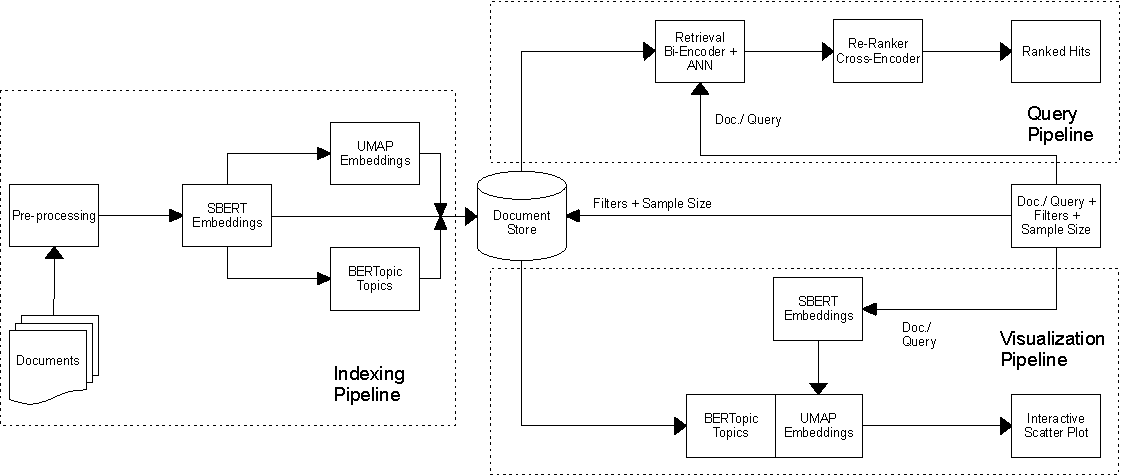
\includegraphics[width=\linewidth]{./assets/system_architecture}
	\caption{\textbf{MapIntel architecture}. Composed of three main pipelines: Indexing, Query, and Visualization}
	\label{system_architecture}
\end{figure}

\subsection{Indexing} \label{indexing}
In this work we decided to focus on how NLP, particularly sentence embeddings, could help organize, explore, and retrieve text documents in the CI domain. Thus, we have not developed the precedent tasks of data collection and pre-processing as much as we believe they are independent of the system and can be easily integrated with it. Nevertheless, it is essential to point out that the system's quality is extremely reliant on these steps, as if we feed it non-ideal data, we will get non-ideal results. MapIntel is nothing but a set of tools to facilitate the exploration and understanding of a corpus, and it will not give useful insights if the data is not useful itself.

Once new documents are fed to the system, their respective embeddings are computed. This process is the basis of our work as it allows the encoding of the semantic identity of the document onto a vector of a given dimensionality. This semantic identity describes the subject of the document, and can be used to compare documents between each other \textit{i.e.}, documents with the same subject will be close in the semantic space and vice-versa. We used SBERT \citep{reimers2019}, a derivative of the Transformer-based BERT model, to embed the documents using a pre-trained encoder trained on reducing the distance between queries and relevant results in the MS MARCO dataset \citep{bajaj2018}. This step produced vectors of 768 dimensions, which we then reduced to 2 dimensions using the Uniform Manifold Approximation and Projection (UMAP) \citep{mcinnes2020} algorithm. UMAP constructs a topological representation of the high and low dimensional data. Its goal is to minimize their cross-entropy, which measures the difference between the two representations, by adjusting the low-dimensional representation. This aspect is another crucial component of MapIntel as it allows the organization and localization of the entire document collection in a 2-dimensional map, which can be used to explore and interact with the data. We opted to use UMAP over other dimensionality reduction techniques because of its improved map quality, reduction in time required to produce the output map, support for larger data set sizes, and, most importantly, its ability to update the output map with new data without having to rebuild it \citep{mcinnes2020}.

We also applied a topic modeling technique called BERTopic \citep{grootendorst2020}, based on the work of \citet{angelov2020}. Topic modeling unveils the latent semantic structure of the data and unlike some of the classical techniques such as Latent Dirichlet Allocation \citep{blei2003} and Probabilistic Latent Semantic Indexing \citep{hofmann1999}, BERTopic leverages the SBERT embeddings and their capacity to encode the semantic attributes of a document to find the most representative topics of a corpus. BERTopic clusters the documents using Hierarchical Density-Based Spatial Clustering of Applications with Noise (HDBSCAN) \citep{mcinnes2017} to find the densest areas of the semantic space while identifying outliers. To overcome the sparsity of the high-dimensional space and the obstacles it creates in finding dense clusters, UMAP is used to reduce the embeddings to a lower dimension (5 dimensions by default) prior to the clustering stage, this UMAP is separate from the one we use to visualize the corpus on 2 dimensions. The primary assumption behind BERTopic is that each dense area in the semantic space is generated by a latent topic shared among the documents that comprise it. Finally, a class-based variant of TF-IDF \citep{jones1972} (c-TF-IDF) is used to extract an importance value of each word for each cluster, which can be used to represent each topic as the set of its most important words. Another advantage of BERTopic over the classical approaches is that we can reduce the number of topics obtained by iteratively comparing the c-TF-IDF vectors, merging the least common topic with its most similar topic, and re-calculate the c-TF-IDF vectors, giving us the option to choose the number of topics.

Finally, we loaded the documents including their metadata, SBERT embeddings, UMAP embeddings, and topics into a database. We used Open Distro for Elasticsearch\footnote{\href{https://opendistro.github.io/for-elasticsearch/}{opendistro.github.io/for-elasticsearch}} — an open-source, RESTful, distributed search and analytics engine based on Apache Lucene\footnote{\href{https://lucene.apache.org/}{lucene.apache.org}} — to store the data, organize it in an index, and perform full-text search on it. We can think of the described approach as an Indexing Pipeline — Figure \ref{indexing_pipeline} — that extracts new raw documents from a data source, pre-processes and manipulates them, stores the results in a database, and indexes the documents for future search tasks.

\begin{figure}[H]
	\centering
	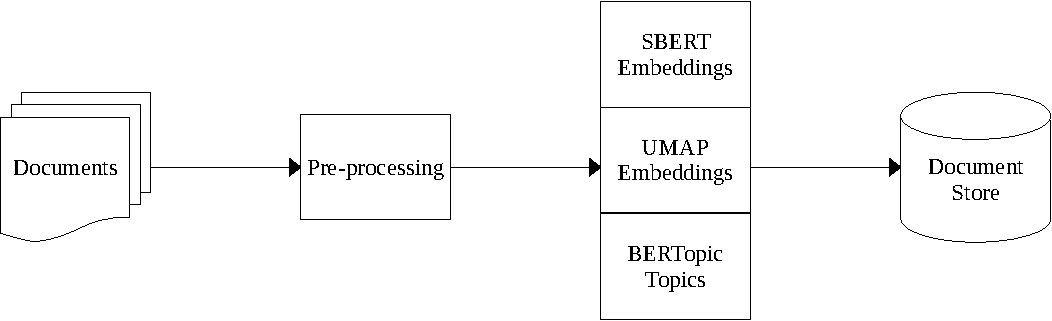
\includegraphics[width=\linewidth]{./assets/indexing_pipeline}
	\caption{\textbf{Indexing pipeline}. Documents flow through a pre-processing step, followed by an inference step where their SBERT embeddings, UMAP embeddings and BERTopic topics are computed and indexed into a Database for future search tasks.}
	\label{indexing_pipeline}
\end{figure}

\subsection{Query} \label{query}
Finding meaningful information within a large amount of data is a sizable part of the CI task. The ability to retrieve relevant documents from a large collection of news articles through natural language queries empowers the CI analyst with an easy and intuitive interface to scan the environment.

MapIntel provides a search functionality based on Open Distro for Elasticsearch and its $k$-Nearest Neighbor ($k$NN) Search module. By utilizing the $k$NN module, we can leverage the SBERT embeddings by projecting the query string onto the same semantic space as the corpus and computing its $k$-nearest neighbors \textit{i.e.} finding the $k$ documents whose embedding vectors are closest to the query embedding vector, according to some predefined similarity metric. Since the embedding vectors encode the semantic identity of each document, this method provides semantically relevant results for a given query. Furthermore, the $k$NN module delivers a highly performant and scalable similarity search engine by leveraging Elasticsearch’s distributed architecture and by implementing Approximate Nearest Neighbors (ANN) search based on Hierarchical Navigable Small World Graphs \citep{malkov2018}. The $k$NN module can also be combined with binary filters that help the user obtain focused results based on characteristics of the documents such as publication date and topic. These filters are applied directly to the database, reducing the search space as a result and improving the subsequent search time.

Once again, we can think of the search functionality as a pipeline, illustrated in Figure \ref{query_pipeline}, where we feed a query string and some binary filters, and obtain documents ordered by their relevance to the query. We employ a Retrieve and Re-rank pipeline based on the works of \citet{nogueira2020a, kratzwald2019} composed by a "Retrieval Bi-Encoder + ANN" node that performs a semantic search using Elasticsearch’s $k$NN module as described above, and by a "Re-Ranker Cross-Encoder" node consisting of a BERT model fine-tuned on the MS MARCO dataset that receives a document and query pair as input and predicts the probability of the document being relevant to the query.

The pipeline works by taking advantage of the characteristics of both nodes. The Bi-Encoder, together with ANN search, can retrieve fairly relevant candidates while dealing efficiently with a large collection of records. The Cross-Encoder is not as efficient since it has to be performed independently for each document, given a query. However, since attention is performed across the query and the document, the performance is higher in the second node \citep{humeau2019}. Therefore, we combined both nodes by retrieving a large set of candidates from the entire collection using the Bi-Encoder, and filtering the most relevant candidates with the Cross-Encoder while removing noisy results.

With this pipeline, we can provide relevant documents to the user given a query and binary filters while ranking them according to a relevancy score. The pipeline is efficient and uses the SBERT embeddings and the Elasticsearch architecture. As an additional feature, we can input a document instead of a query, allowing us to search for semantically similar documents within the collection.

\begin{figure}[H]
	\centering
	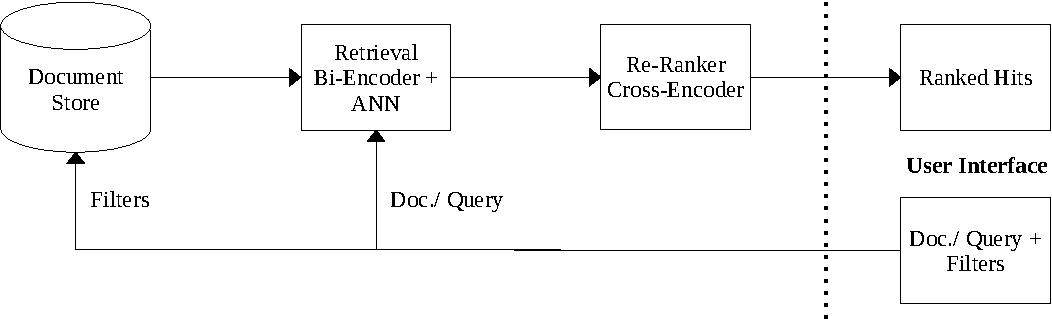
\includegraphics[width=\linewidth]{./assets/query_pipeline}
	\caption{\textbf{Query pipeline}. Given a user query or selected document, its SBERT embedding is inferred and the closest neighbors are computed while a set of binary filters is used to reduce the search space. Following, a Cross-Encoder BERT model is used to re-score the neighbors from the previous step, and they are retrieved together with their similarity score.}
	\label{query_pipeline}
\end{figure}

\subsection{Visualization}
We developed a visual interface that organizes and displays the documents to facilitate the environment scanning task, giving the user the ability to browse the data and zoom on particular regions of the semantic space. The interface uses the UMAP algorithm to reduce the dimensionality of the original semantic space to a 2-dimensional representation that reliably preserves the original topology.

The methodology employed to produce the interface is described in Figure \ref{vis_pipeline}. It begins by taking the same inputs passed to the Query pipeline: a query, and a set of filters. The common inputs create a connection between the two modules — when the user queries the database, the query text is projected onto the 2-dimensional map and the filters define which documents are displayed in the map. In this way, the map can be seen as a graphical extension of the searching mechanism, where the relevant results reside in the neighborhood of the query, giving the user some insight into how the results are obtained. In addition to the common inputs, we require a relative sample size that defines the percentage of randomly chosen documents (after applying the filters) to be displayed in the map. This step is necessary as interaction with the map is hindered by a large number of data points, resulting in a slow and unresponsive experience. Notice that the sample size does not affect the query results, as the search is always performed on the entire collection.

The filters and sample size are used to select the documents to be displayed from the database to produce the interactive scatter plot. We compute the SBERT embedding of the query, followed by its UMAP embedding, thus being able to locate the query in the same space as the documents. An advantage of these two models is that we can efficiently produce embeddings of new text without having to re-train them, making this process quite fast. Once we have the UMAP embedding of the query, we join it with the pre-computed embeddings of the documents from the Indexing pipeline, and we produce the interactive map.

The map provides a means to explore the documents and the different semantic cohorts present within the collection. We color-code the points with the documents' topics identified in the Indexing stage, allowing us to visualize the latent semantic structure of the data, and when hovered, the points display their corresponding title and content attributes.

\begin{figure}[H]
	\centering
	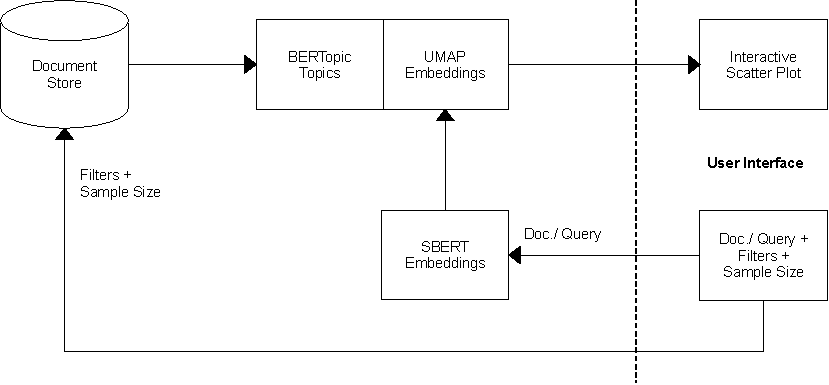
\includegraphics[width=\linewidth]{./assets/vis_pipeline}
	\caption{\textbf{Visualization pipeline}. Given a user query or selected document, its SBERT and UMAP embedding are inferred while a set of binary filters and a sample size is used to reduce the number of documents retrieved. Finally, the selected documents' topics and 2-dimensional embeddings, together with the query embedding, are displayed in an interactive scatter plot.}
	\label{vis_pipeline}
\end{figure}

\section{Evaluation}
Our methodology addresses the issues of information dispersion and overload impacting the CI analysts' tasks. The proposed system provides searching and browsing capabilities, contributing to an easier understanding of the business environment by supporting analysts in seeking specific information while promoting undirected information encountering. In this section, we elaborate our choices in the design of the MapIntel system with the results of our experiments and analyze the different components of the system individually.

\subsection{Experimental Setup}
We evaluate our system quantitatively using the 20 newsgroups \citep{pedregosa2011} dataset and the document labels provided. This dataset consists of around 18,000 newsgroups posts on 20 topics divided into 6 main groups: "Computer," "Recreation," "Science," "Miscellaneous," "Politics," and "Religion." We opted to use this dataset because of the presence of labels that describe the semantic meaning of each document, allowing us to have a reference which we can compare the identified topics with.

Given the inherent difficulty of evaluating the system in its entirety, we decided to deal with each component separately, however since every component of our system depends on the vector representation of the documents, we cannot guarantee an orthogonal evaluation of the components. We focus our experiments in comparing 2 of the main components of the MapIntel system: the Topic Model and the Sentence Embedding. The following algorithms are compared in our paper:
\begin{itemize}
	\item \textbf{Sentence embeddings}
	      \begin{enumerate}
		      \item \textbf{Paragraph Vector Model (or Doc2Vec)} \citep{le2014}: an unsupervised algorithm that learns both word and document vectors by minimizing the error of predicting the next word in a paragraph (a variable-length piece of text) given the paragraph and previous word vectors;
		      \item \textbf{SBERT}: a derivative of the Transformer-based BERT model, to embed the documents using a pre-trained encoder trained on reducing the distance between queries and relevant results in the MS MARCO dataset;
	      \end{enumerate}
	\item \textbf{Topic modeling}
	      \begin{enumerate}
		      \item \textbf{LDA}: a generative probabilistic model of a corpus in which each document is modeled as a finite mixture over an underlying set of topics, and each topic is characterized by a distribution over words;
		      \item \textbf{BERTopic}: a cluster-based topic model that unveils the latent document-topic distribution responsible for the existing groups of documents in a semantic vector space;
		      \item \textbf{Contextualized Topic Model (CTM)} \citep{bianchi2021}: combines contextualized representations (like SBERT) with neural topic models resulting in more meaningful and coherent topics;
	      \end{enumerate}
\end{itemize}

We use three main metrics to guide our model comparison:
\begin{itemize}
	\item \textbf{$k$NN classifier accuracy for the UMAP projections}: evaluate the quality of the two-dimensional projections by inferring their labels using a $k$NN classifier and computing its Accuracy for multiple values of $k$ \citep{mcinnes2020}. We present the average Accuracy over the range of $k$ values we tried: 10, 20, 40, 80, 160.
	\item \textbf{Normalized Mutual Information (NMI) for the topic assignments}: information theoretic based measure that tells us how much knowing about the topics of the documents reduces our uncertainty about the original labels and vice-versa \citep{vinh2009}. The NMI ranges between 0 and 1 where the former corresponds to no mutual information, and the latter indicates perfect correlation. The higher the value of this metric, the better we can capture the true topical nature of the documents, reflected by their labels, with the assigned topics.
	\item \textbf{Topic coherence}: measure the quality of the words that describe each topic by applying the $C_v$ metric \citep{roder2015} indicating whether the words that compose a given topic support each other. This metric is shown to be correlated with human ratings on understandability of topic descriptions, given as word sets, and it ranges between -1 and 1, where the former corresponds to incoherent topic descriptions, and the latter indicates a coherent topic description.
\end{itemize}

% l and g are the GMM densities. Basically we choose the hyperparameter that has the largest likelihood of belonging to the density l in relation to g
We performed hyperparameter tuning using a multi-objective approach to optimize the three metrics specified previously. We used the Tree-structured Parzen Estimator (TPE) algorithm \citep{bergstra2011, ozaki2020} for sampling the hyperparameter space at each trial $t$ of the optimization process. Contrarily to random search, TPE samples values $x_t^\alpha$ for each hyperparameter $\alpha$ by fitting one Gaussian Mixture Model (GMM) $l(x^\alpha)$ to the set of values associated with the best objective scores in past observed trials, and another GMM $g(x^\alpha)$ to the remaining values. It then chooses the hyperparameter value $x_t^\alpha$ drawn from $l(x^\alpha)$ that maximizes the ratio $\frac{l(x^\alpha)}{g(x^\alpha)}$. For each trial, we evaluated the sampled hyperparameters using a 5-fold cross-validation approach where the folds preserve the percentage of samples of each class. In total, 100 trials were evaluated.

\subsection{Results}
Our results based on the setup described above are shown in Table \ref{table2}. For each trial, we report the average results and standard deviations over the cross-validation folds. The table contains the best trials for each of the Topic/Embedding model combinations according to the average of the three objective metrics, which we applied MinMax scaling to avoid any impact of the metrics scale on the choice of the best model. We can see that the combination that uses BERTopic and SBERT outperform the others with respect to both NMI and $C_v$ while having a within standard deviation $k$NN Classifier Accuracy to the best value. Another interesting observation is that combinations using SBERT have generally better results. To facilitate results reproduction efforts, we open-sourced the code developed for the experiments at \href{https://github.com/NOVA-IMS-Innovation-and-Analytics-Lab/mapintel_research}{github.com/NOVA-IMS-Innovation-and-Analytics-Lab/mapintel\_research}.

\begin{table}[H]
	\centering
	\resizebox{0.95\textwidth}{!}{%
		\begin{tabular}{@{}llYYYY@{}}
			\toprule
			\textbf{Topic Model} & \textbf{Embedding Model}     & {MinMax Average} & {NMI}             & {Topic Coherence $C_v$} & {$k$NN Classifier Accuracy} \\ \midrule
			BERTopic             & \multicolumn{1}{l|}{Doc2Vec} & 0.50             & 0.11(1)           & 0.72(2)                 & 0.16(1)                     \\
			BERTopic             & \multicolumn{1}{l|}{SBERT}   & \bfseries 0.94   & \bfseries 0.36(3) & \bfseries 0.76(8)       & 0.36(1)                     \\
			CTM                  & \multicolumn{1}{l|}{Doc2Vec} & 0.56             & 0.23(2)           & 0.55(2)                 & 0.24(3)                     \\
			CTM                  & \multicolumn{1}{l|}{SBERT}   & 0.70             & 0.33(2)           & 0.58(2)                 & 0.28(4)                     \\
			LDA                  & \multicolumn{1}{l|}{Doc2Vec} & 0.58             & 0.25(3)           & 0.53(3)                 & 0.25(1)                     \\
			LDA                  & \multicolumn{1}{l|}{SBERT}   & 0.71             & 0.26(3)           & 0.53(3)                 & \bfseries 0.37(5)           \\ \bottomrule
		\end{tabular}%
	}
	\caption{Hyperparameter tuning best trials per topic and embedding model according to the MinMax average of the multiple objective metrics.}
	\label{table2}
\end{table}

Additionally, we present the UMAP 2-dimensional maps of the documents in the 20 newsgroups dataset. Figure \ref{umap_train_plots} shows the comparison between the distribution of the original labels and the topics assigned by the best performing model according to the MinMax average score for the train data (see Table \ref{best_hyperparameters} for exact hyperparameter values). Likewise, Figure \ref{umap_test_plots} shows the same comparison for the test data and demonstrates the ability of the model to generalize to unseen samples. We can see that the identified topical cohorts are mostly matching with the original groups, indicating that the embeddings have learned the original labels in a fully unsupervised way. Additionally, it is possible to see that semantically similar topics are located close to each other in the map. This is the case of all the computation related topics such as \emph{window.server.windows.motif.display} and \emph{format.files.graphics.file.gif}. Finally, there is also an agreement between the topic meaning given by the top 5 words describing the topics and the original label description. For example, the same points that have the label \emph{sci.space} also have the topic \emph{space.launch.nasa.orbit.shuttle}. Figure \ref{umap_train_plots_zoom} in the appendix shows how much correspondence there is both in terms of labels and positioning for technological-related documents - we can see how the distribution of the original label \emph{comp.graphics} matches the distribution of the topic \emph{format.files.graphics.file.gif}, likewise \emph{comp.windows.x} matches \emph{window.server.windows.motif.display}, and \emph{sci.electronics} matches \emph{amp.radio.powed.voltage.use}, whereas the remaining original labels are lost, giving birth to new, and more semantically coherent, groups of documents (note how the distribution of the original label \emph{comp.sys.ibm.pc.hardware} is very dispersed, even overlapping with other groups and how the distribution of the topics occupying the same region is very clear and compact).

\begin{figure}[H]
	\centering
	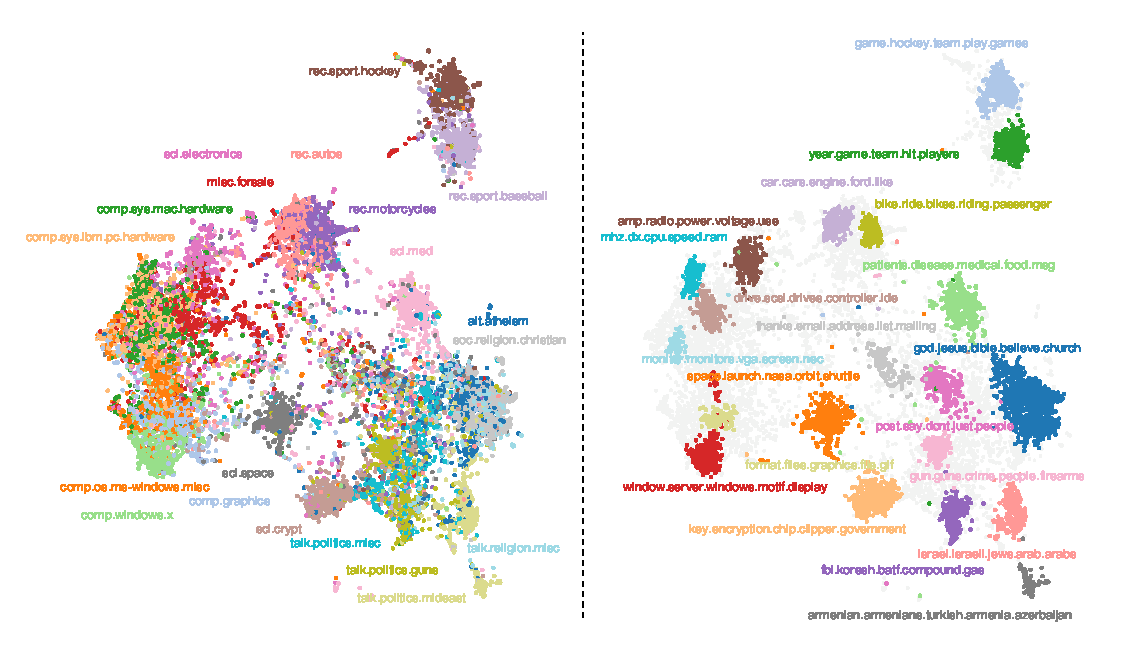
\includegraphics[width=\linewidth]{./assets/umap_train_plots}
	\caption{Comparison between UMAP planes of \textbf{train data} with original (left) and topic labels (right).}
	\label{umap_train_plots}
\end{figure}

\begin{figure}[H]
	\centering
	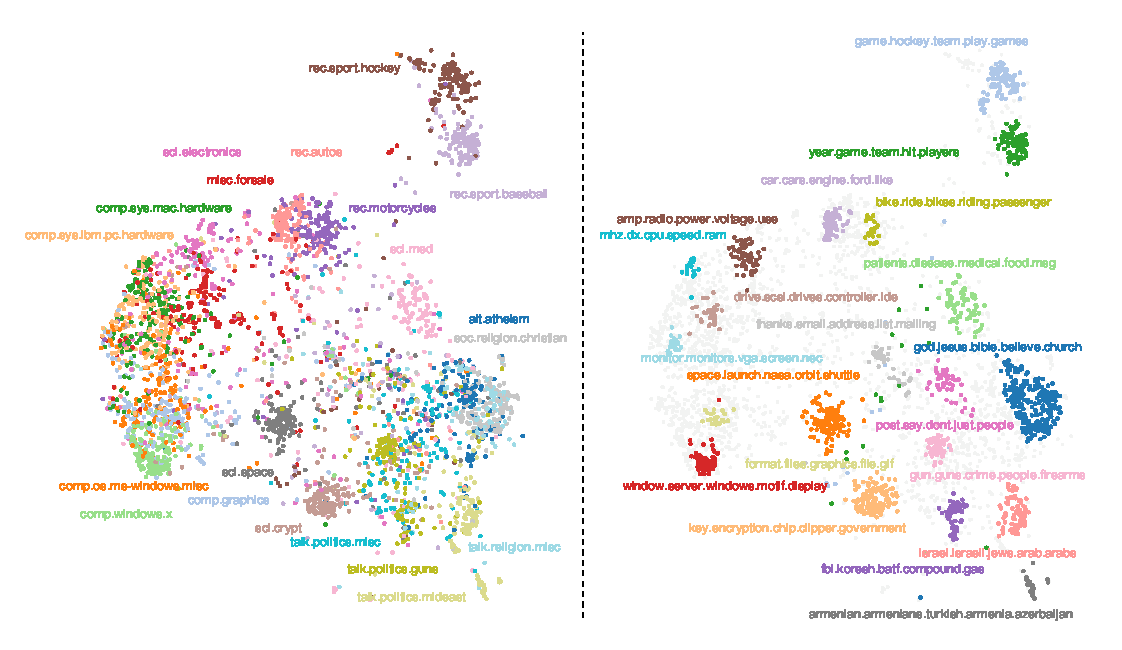
\includegraphics[width=\linewidth]{./assets/umap_test_plots}
	\caption{Comparison between UMAP planes of \textbf{test data} with original (left) and topic labels (right).}
	\label{umap_test_plots}
\end{figure}

An important characteristic of BERTopic is that it is able to identify noise, leading to a topic assignment where a portion of the observation are classified as outliers. This produces a cleaner map to explore the documents at the loss of samples that are not given a topic. In Figure \ref{umap_train_plots} (left) the percentage of documents classified into the aforementioned category is 51.4\% - these are the light grey points scattered across the map.

\section{Case Study}
This use case is based on a real-world example, related to the recurrent tasks that the intelligence analysts at AICEP - Portuguese Trade \& Investment Agency have to perform. AICEP “is a government business entity, focused in encouraging the best competitive foreign companies to invest in Portugal and in contributing to the success of Portuguese companies abroad in their internationalization processes or export activities.” Given this mandate AICEP needs to monitor the world news and make sure it is updated with world events. Additionally, analysts at AICEP are called upon to produce reports on specific markets and industries, in order to guide the Portuguese state's diplomatic efforts and private company investments. These reports are pre-formatted, however the use and integration of text data remains a challenge. This is unfortunate as recent news and text documents allow a more detailed understanding of specific problems and nuances that are difficult to capture in an alphanumeric data table. The objective of this use case is to show how MapIntel can be used to mitigate this limitation and allow the inclusion of relevant text data in the report.

In this case study, we will show the most important tools that the MapIntel system offers to explore and select relevant documents to include in a market or industry report. These tools allow the analyst to screen the news and select those that are relevant to include in the report. This process cannot be strictly seen as an information retrieval process, in fact it is much more an exploration process, in which the analyst’s criterion plays a crucial role. The process usually starts with a natural language query that the analyst defines based on his/her knowledge of the market or industry. The query is used by the system as the seed in the process of exploring the corpora. The query is projected onto the two-dimensional surface produced by MapIntel, and the neighbor documents are defined in the semantic space, thus generating a number of candidate results relevant for the report. From this starting position the analyst can interact visually with the results and the entire corpus, and guide his/her interest with successive queries, focusing in the most interesting/promising instances to include in the report.

To evaluate the MapIntel system with real data, we gathered news articles from multiple international sources with the use of an API\footnote{\href{https://newsapi.org/}{newsapi.org}}. As already stated, there are multiple sources of CI, and different information can be obtained from these. \citet{dey2011} shows in Table \ref{ci_sources} what kind of information can be acquired from these sources, particularly the ones that are easily available through the web. We decided to work mainly with news articles as they provide a general and accessible means of information about the environment, however, our methodology is easily extensible to data from different sources.

\begin{table}[H]
	\centering
	\resizebox{0.9\textwidth}{!}{%
		\begin{tabular}{@{}ll@{}}
			\toprule
			\textbf{Type of Competitive Intelligence}          & \textbf{Web Resources}                             \\ \midrule
			People event                                       & News, company web-sites                            \\
			Competitor strategies, Technology investment, etc. & News, Discussion forum, Blogs, Patent search sites \\
			Consumer sentiments                                & Review sites, Social networking sites              \\
			Promotional events and pricing                     & Social networking sites                            \\
			Related real-world events                          & News, Social networking sites                      \\ \bottomrule
		\end{tabular}%
	}
	\caption{Competitive intelligence resources on the web \citep{dey2011}.}
	\label{ci_sources}
\end{table}

The API employed retrieves news articles and their metadata, including attributes such as source, author, title, description, content, category, URL, and publication date and time. We used this API to feed the system with updated data on a schedule while focusing on articles written in English from a set of predefined categories (business, entertainment, general, health, science, sports, technology). The system was fed with a total of 334,925 articles during the period between October 2020 and June 2021.

Due to API limitations, the retrieved data has its content truncated to 200 characters. To overcome this, we treat a single document unit as the concatenation of title, description, and content, providing us a semantically loaded piece of text that we can use for testing the system. Despite this limitation, we give the user the possibility of accessing the full article through its URL. We ensure that each document is unique, is written in English, and doesn't have any HTML tags or any strange pattern.

Once the data is cleaned, it follows the Indexing pipeline \ref{indexing_pipeline}, so it can be used downstream by the Query pipeline \ref{query_pipeline} and the Visualization pipeline \ref{vis_pipeline}.

\begin{figure}[H]
	\centering
	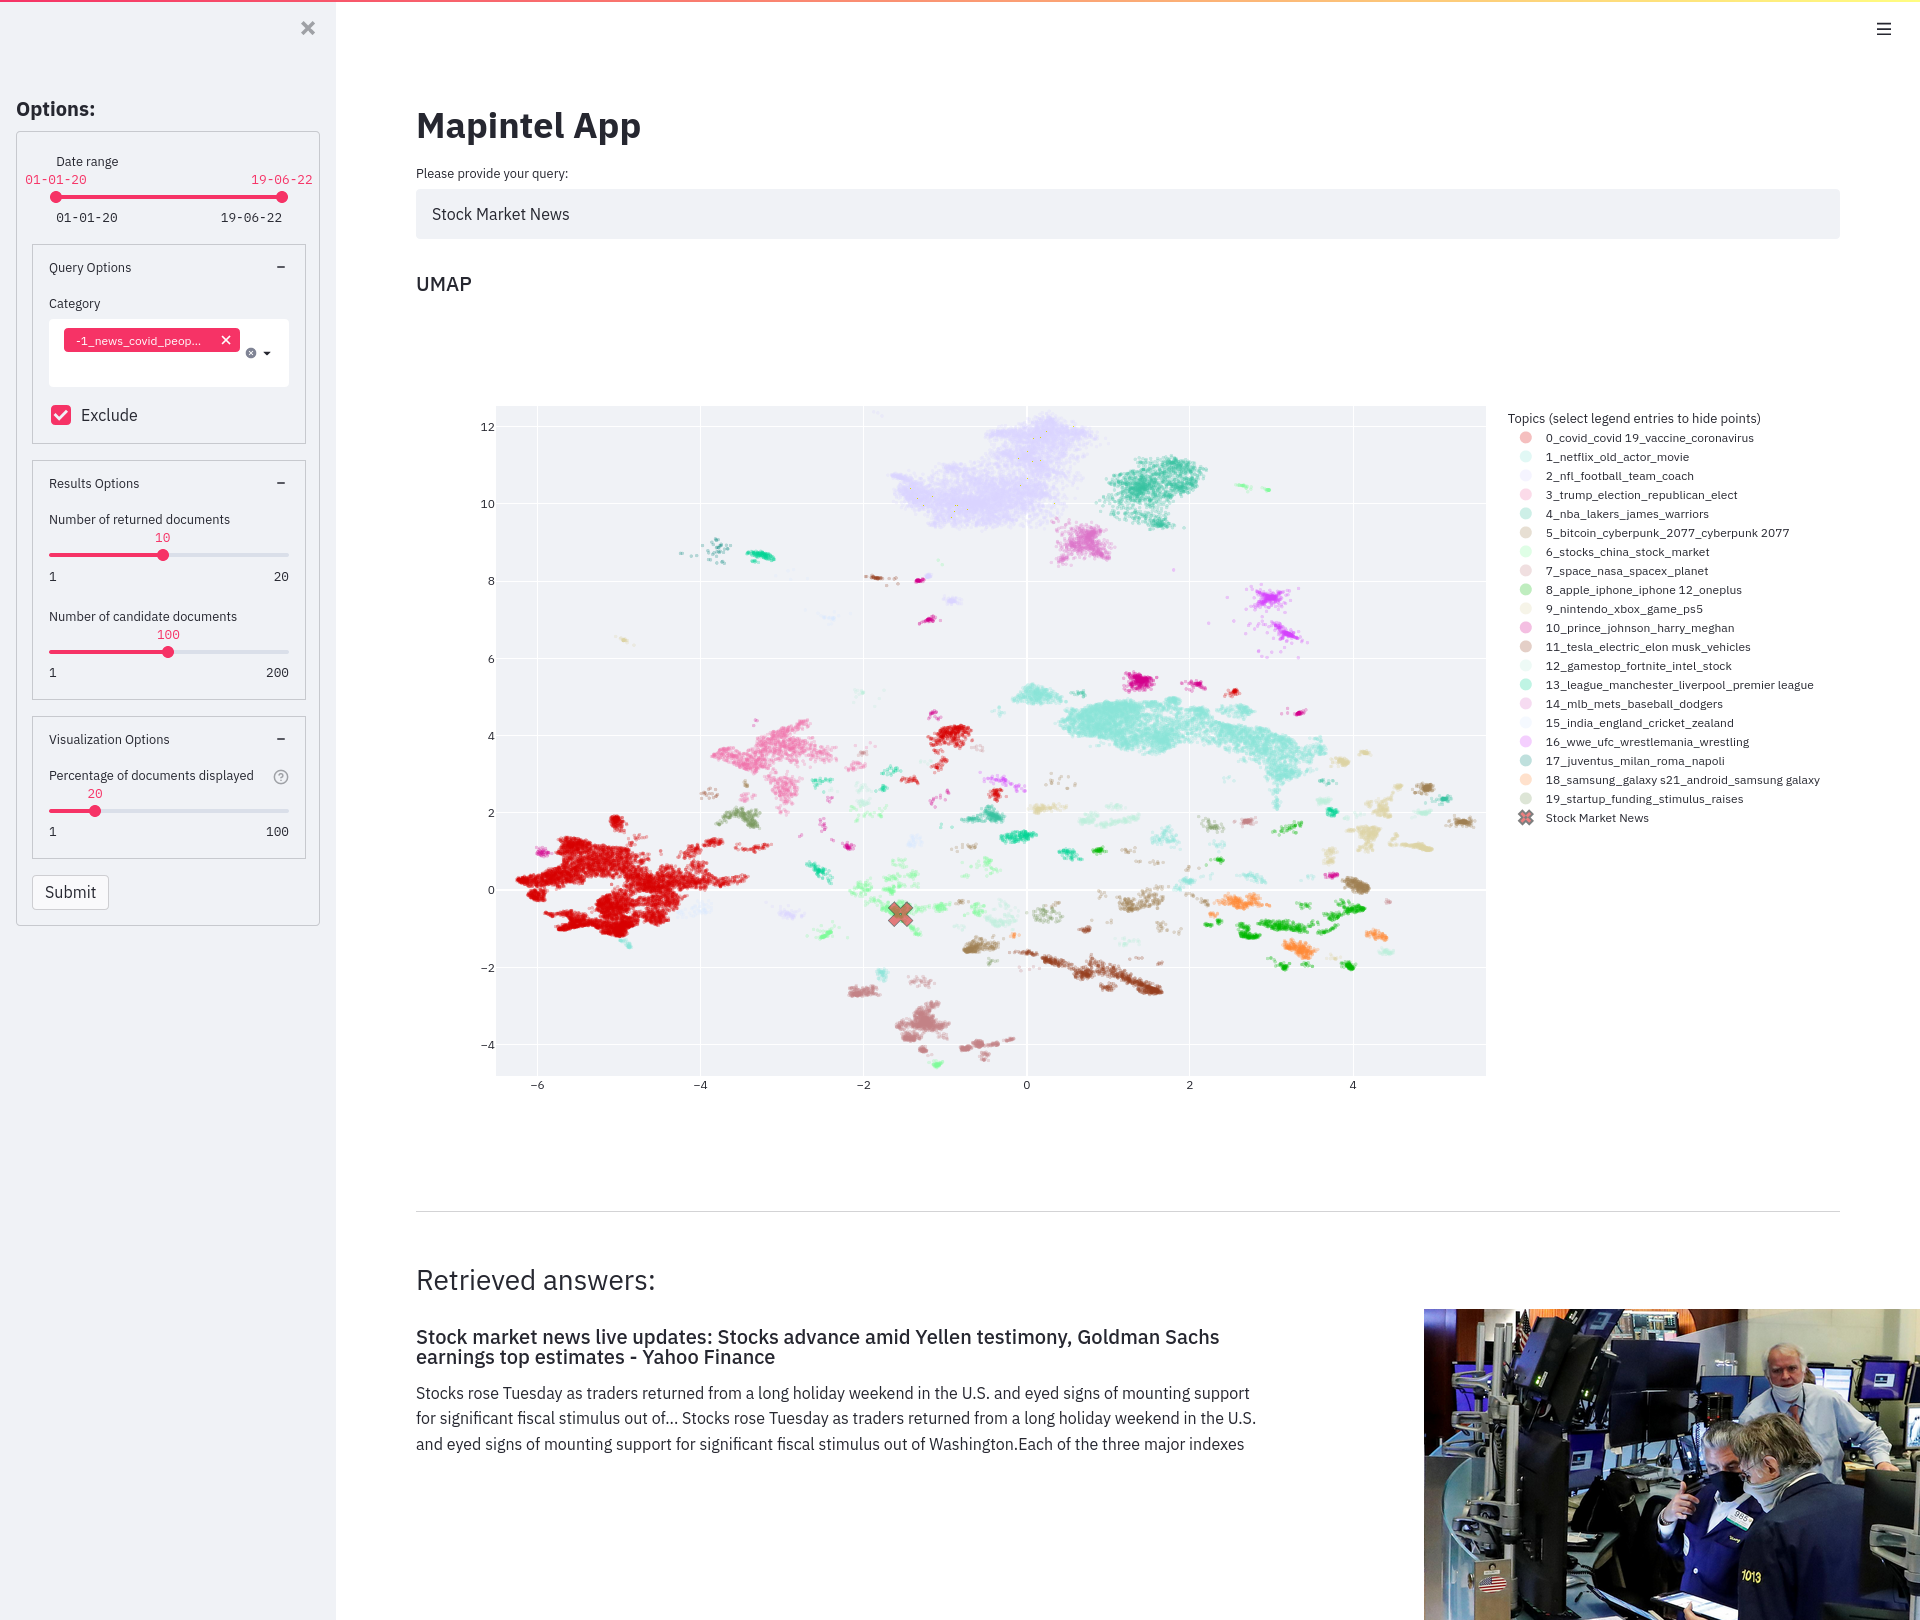
\includegraphics[width=0.8\linewidth]{./assets/ui_screenshot}
	\caption{\textbf{MapIntel webapp interface}. Composed of four main components: search box, interactive scatter plot, parameter sidebar, and list of results.}
	\label{app_ui}
\end{figure}

We also built a simple web application in Python based on the MapIntel system. The web application is containerized and composed of three main modules: an Elasticsearch instance container that stores and indexes the documents, their metadata, their topics and their embeddings, a container responsible for all the computations involved in the three pipelines of the system that communicates with the user interface through a FastAPI\footnote{\href{https://fastapi.tiangolo.com/}{fastapi.tiangolo.com}} server providing the necessary endpoints, and a third container consisting of a Streamlit\footnote{\href{https://streamlit.io/}{streamlit.io}} application that interacts with the data through HTTP requests. For transparency, the code used for the web application is made public at \href{https://github.com/NOVA-IMS-Innovation-and-Analytics-Lab/mapintel_project}{github.com/NOVA-IMS-Innovation-and-Analytics-Lab/mapintel\_project}.

We highlight the user interface of the app in Figure \ref{app_ui}. It is composed of 4 main components: a \textbf{search box} at the top of the page that the user can use to write any natural language query, an \textbf{interactive scatter plot} that shows the UMAP projection of the document embeddings and allows the exploration of the corpus, a \textbf{sidebar} at the left where the user can specify any additional parameter or binary filter to the query and map, and a \textbf{list of results} at the bottom that contains the documents with the highest scoring for the specified query.

The app enables information searching by receiving a query through the search box together with the filters and parameters selected in the sidebar. This allows the CI analyst to write queries in Natural Language while having a finer control of the results through sidebar parameters like including or excluding specific topics and specifying a date range. We show in Table \ref{query_results} some query examples (without any filters) a CI analyst could make and their respective results. We can see that the results are semantically relevant to the query provided.

\begin{table}[H]
	\centering
	\resizebox{0.9\textwidth}{!}{%
		\begin{tabularx}{\linewidth}{lXl}
			\toprule
			\textbf{Query}                            & \textbf{Top 3 Results (Title)}                                                                              & \textbf{Score} \\  \midrule
			\multirow{3}{*}{"Suez Canal World Trade"} & Suez Canal blockage felt across the world as trade comes to a pause.                                        & 4.90           \\
			                                          & Suez Canal ship partially refloated after huge effort to unblock key global trade route.                    & 4.70           \\
			                                          & Egypt 'seizes' container ship over \$1bn Suez claim.                                                        & 4.42           \\  \midrule
			\multirow{3}{*}{"Indian Elections"}       & India elections: Modi party defeated in West Bengal battleground - BBC News.                                & 5.36           \\
			                                          & At 103, India's first voter casts vote in Himachal panchayat radish polls.                                  & 4.77           \\
			                                          & Vote count in five Indian states under way as pandemic rages.                                               & 4.44           \\  \midrule
			\multirow{3}{*}{"Oil Prices"}             & Oil prices near 2-year highs above \$70 as investors expect OPEC+ to confirm its supply policies.           & 7.63           \\
			                                          & Oil Prices Rally Towards \$70 As Demand Outlook Improves - OilPrice.com.                                    & 7.62           \\
			                                          & Oil prices to reach \$72 by summer: Goldman Sachs - Fox Business.                                           & 7.45           \\  \midrule
			\multirow{3}{*}{"Myanmar Coup"}           & Myanmar Coup: With Aung San Suu Kyi Detained, Military Takes Control - NPR.                                 & 8.03           \\
			                                          & Myanmar's military has detained leader Aun San Suu Kyi in a coup. Here's what you need to know - CNN.       & 8.03           \\
			                                          & News24.com | Myanmar military stages coup and declares state of emergency, detains leader Aung San Suu Kyi. & 7.94           \\  \bottomrule
		\end{tabularx}%
	}
	\caption{Example queries and their top 3 results and respective relevancy scores. The results are computed according to the methodology described in \ref{query}.}
	\label{query_results}
\end{table}

An additional feature of the app is the ability to browse documents through the scatter plot. This visualization shows the 2-dimensional UMAP projection of the 768-dimensional embeddings of the documents. It can be used by the analyst to explore the document collection and the underlying thematic groups. The map can be interacted with by zooming, panning and hovering specific regions and documents, allowing the analyst to see the content of each data point. A representation of the hovering capability and a more detailed image of the document map can be seen in Figure \ref{app_map}. In addition, we integrate the \emph{searching} and \emph{browsing} modules of the system by plotting the query embedding in the UMAP plane - represented with an "X" shaped marker -, allowing a visual exploration of the relevant results \emph{i.e.} the data points close to the query. Finally, we allow searching of similar documents by providing the option to click on any point in the map and obtain their most similar documents in the list of results below. We found that this feature enhances exploration and finding of relevant documents.
% TODO: the last feature of similar document search isn't yet implemented but should be pretty straightforward

\begin{figure}[H]
	\centering
	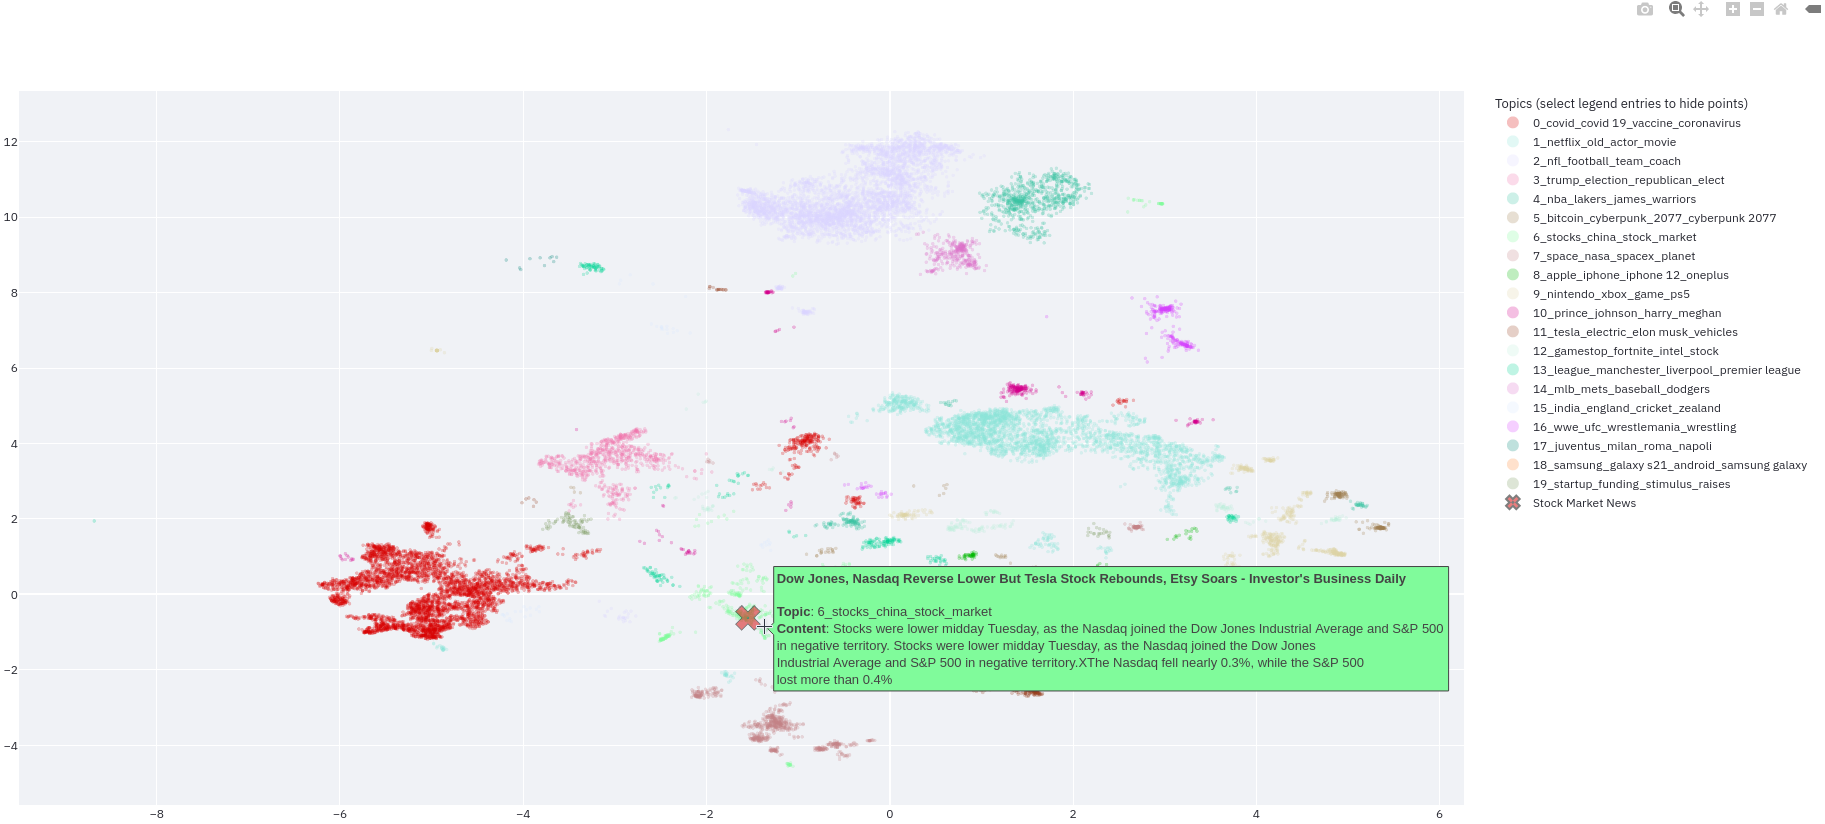
\includegraphics[width=0.8\linewidth]{./assets/map_screenshot}
	\caption{\textbf{UMAP projection of the corpus}. The documents' SBERT embeddings are projected on two dimensions with UMAP and the data points are colored according to their assigned topic. The map can be used interactively by zooming, panning, hovering, and selecting points. On hovering, the document text and some metadata is displayed and on selection the document is queried against the rest of the corpus. The query is marked with an "X" in the map.}
	\label{app_map}
\end{figure}

Besides the searching and browsing functionality, the system can also organize the documents into semantically similar cohorts and automatically label them. This is achieved with the help of topic modeling - particularly BERTopic - and the resulting topic labels can be seen in Table \ref{topic_labels}. The topic labels can be particularly useful to the analyst to understand the different subjects covered by the corpus at a glance. In addition, by looking at Figure \ref{app_map} we can notice that these topics represent clusters of documents in the semantic space, which confirms the main assumption that semantically similar documents have similar embeddings.

\begin{table}[H]
	\centering
	\resizebox{0.8\textwidth}{!}{%
		\begin{tabular}{@{}Sll@{}}
			\toprule
			\textbf{Topic Number} & \textbf{Topic Words}                         & \textbf{Topic Coherence} \\  \midrule
			-1                    & - (outliers)                                 & -                        \\
			1                     & covid, covid 19, vaccine, coronavirus        & 0.644                    \\
			2                     & netflix, old, actor, movie                   & 0.223                    \\
			3                     & nfl, football, team, coach                   & 0.359                    \\
			4                     & trump, election, republican, elect           & 0.12                     \\
			5                     & nba, lakers, james, warriors                 & 1                        \\
			6                     & bitcoin, cyberpunk, 2077, cyberpunk 2077     & 0.336                    \\
			7                     & stocks, china, stock, market                 & 0.413                    \\
			8                     & space, nasa, spacex, planet                  & 0.314                    \\
			9                     & apple, iphone, iphone 12, oneplus            & 1                        \\
			10                    & nintendo, xbox, game, ps5                    & 1                        \\
			11                    & prince, johnson, harry, meghan               & 1                        \\
			12                    & tesla, electric, elon musk, vehicles         & 0.943                    \\
			13                    & gamestop, fortnite, intel, stock             & 0.212                    \\
			14                    & league, manchester, liverpool, premier leagu & 1                        \\
			15                    & mlb, mets, baseball, dodgers                 & 0.356                    \\
			16                    & india, england, cricket, zealand             & 1                        \\
			17                    & wwe, ufc, wrestlemania, wrestling            & 1                        \\
			18                    & juventus, milan, roma, napoli                & 1                        \\
			19                    & samsung, galaxy s21, android, samsung galax  & 1                        \\
			20                    & startup, funding, stimulus, raises           & 0.617                    \\  \bottomrule
		\end{tabular}%
	}
	\caption{Topic labels and respective coherence values. We used the five words with the highest c-TF-IDF score per topic to label them and extracted the coherence value $C_v$ of these words.}
	\label{topic_labels}
\end{table}

\section{Conclusion}
In this paper, we presented MapIntel, a new system for extracting knowledge from large corpora of text documents. MapIntel differentiates from previous systems in that it leverages Transformer-based document embeddings to provide efficient, natural language searching of documents. The use of Transformer-based embeddings allows to harness the semantic attributes of the documents, which can then be explored in a 2-dimensional map, produced using UMAP. Additionally, MapIntel also organizes the documents in topical cohorts, providing yet another framework for the interaction of the user with the corpus. The system is centered around the concept of Information Encountering \citep{erdelez2020}, providing \emph{browsing} and \emph{searching} capabilities to acquire information and promote serendipity. MapIntel is aimed at supporting Competitive Intelligence analysts by providing a tool that facilitates the exploration and monitoring of the competitive environment from textual data.

We detailed the methodology proposed, having evaluated it through a well-defined experimental setup. Furthermore, we showed how the MapIntel system can be used in a real-world case and we developed a web application, applying the proposed methodology while enhancing the interaction with the underlying data through an interactive scatter plot. Finally, we developed and open-sourced the code base of the web application and our experiments, so the work can be easily reproducible and continued.

Our next steps will be to perform a more extensive evaluation of the system with new corpora and develop a case study more closely with CI analysts from AICEP to better understand their needs. Some different directions would be to expand the system to different application domains to test its generality, include multilingual text documents to more easily monitor international events, and provide a way to interact with subsets of documents through manual selection in the interactive map.

\section*{Acknowledgments}
This work was supported by the \emph{Fundação para a Ciência e Tecnologia of Ministério da Ciência e Tecnologia e Ensino Superior} (research grant under the DSAIPA/DS/0116/2019 project).

\bibliographystyle{apalike}
\bibliography{bibliography}

\appendix
\section{Zoom on UMAP plot}
\begin{figure}[H]
	\centering
	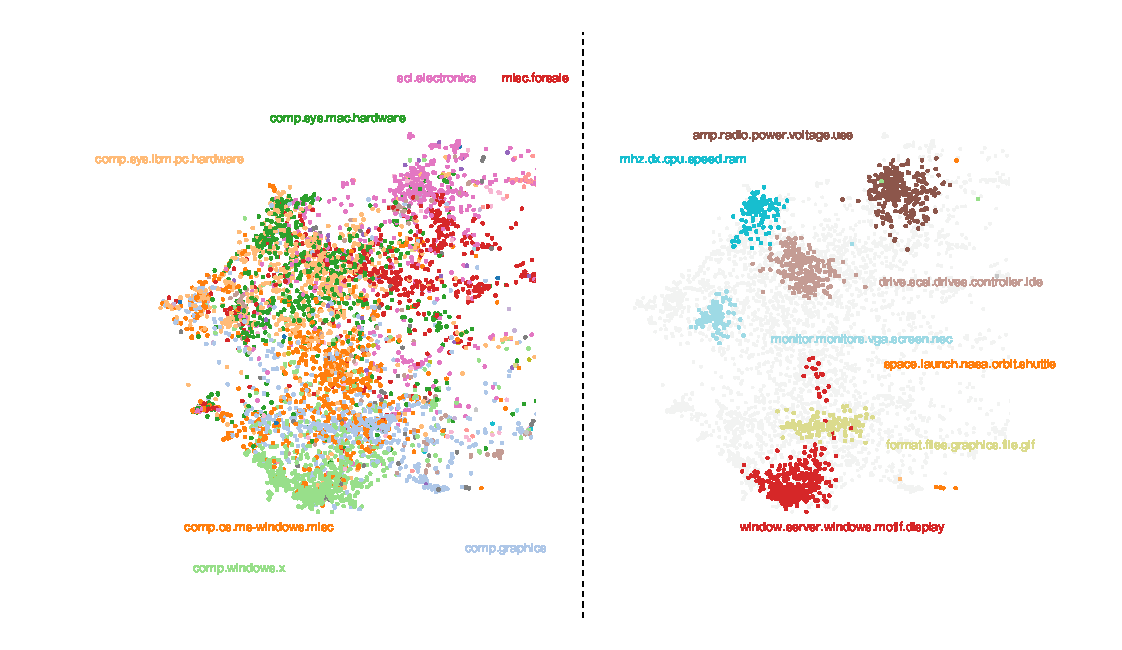
\includegraphics[width=\linewidth]{./assets/umap_train_zoom_plots}
	\caption{Zoom on technological region of UMAP. Comparison between UMAP planes of \textbf{train data} with original (left) and topic labels (right).}
	\label{umap_train_plots_zoom}
\end{figure}

\section{Best hyperparameter configuration}
\begin{table}[H]
	\centering
	\resizebox{0.95\textwidth}{!}{%
		\begin{tabular}{lll}
			\toprule
			\textbf{Model} & \textbf{Hyperparameter}     & \textbf{Value}                                   \\ \midrule
			-              & embedding\_model            & sentence-transformers/msmarco-distilbert-base-v4 \\
			-              & topic\_model                & BERTopic                                         \\
			HDBSCAN        & cluster\_selection\_epsilon & 0.05516517617078291                              \\
			HDBSCAN        & cluster\_selection\_method  & leaf                                             \\
			HDBSCAN        & min\_cluster\_size          & 110                                              \\
			BERTopic       & min\_topic\_size            & 33                                               \\
			UMAP           & metric                      & cosine                                           \\
			UMAP           & n\_components               & 10                                               \\
			UMAP           & n\_neighbors                & 14                                               \\ \bottomrule
		\end{tabular}%
	}
	\caption{Hyperparameter values with the highest MinMax average of NMI, Topic Coherence $C_v$, and $k$NN Classifier Accuracy for training data according to Table \ref{table2}.}
	\label{best_hyperparameters}
\end{table}

\end{document}
